\chapter{Sistema}
En este capitulo se introduce brevemente una serie de conceptos que fueron utilizados para la realizacion del presente proyecto integrador. No se pretende que el lector alcance una comprensión exaustiva de los mismos, sino que tenga las herramientas necesarias para la correcta interpretacion de los capitulos posteriores. De manera paralela se introducen los bloques basicos que formaran parte del sistema planteado.

\section{Sistemas Embebidos y Logica Reconfigurable}
Un Sistema embebido es una combinacion de hardware y software diseñado para realizar funciones dedicadas,generalmente en tiempo real. En algunos casos los sistemas embebidos no actuan de manera independiente y se encuentran integrados en un sistema o producto mayor. 
En la actualidad el 98\% de los microprocesadores fabricados tienen como destino algun sistema embebido mientras que solo el 2\% se destina a microprocesadores de proposito general.

El campo de aplicacion para los sistemas embebidos es muy variado, desde dispositivos portatiles como reproductores MP3 o telefonos celulares, hasta sistemas de control en centrales nucleares. 
No es posible caracterizar los componentes exactos de un sistema embebido ya que existen una gran cantidad de configuraciones posibles, pero dentro de los componentes fundamentales que se encuentran en la mayoria de los sistemas estan:

\begin{itemize}
\item Microprocesador
\item Memoria RAM 
\item Perifericos para Captura de datos
\item Perifericos de Comunicacion.
\end{itemize}





\section{Redes de Computadoras}

*-*-* Esto queda como reserva de datos que despues vmaos a usar****



Uno de los mayores cuellos de botella en los routers lo constituye el cómputo de del prefijo más largo para cada paquete entrante.

Implementar ciertos esquemas de clasificacion en hardware se ve limitado principalmente debido a 2 factores: La cantidad de memoria requerida y lla complejidad creciente de los mismos.

En tanto crece el trafico en las redes se ve la necesidad de implementar esquemas mas complejos de clasificacion.

Dichos esquemas tienen una implementación más sencilla en software. Dichas implementaciones estan ampliamente difundidas en la web.
Esto hace innecesario tener que “adaptarlas” a un HDL. El paso es trivial (corregir esta redaccion)

\section{FPGA}
Son dispositivos lógicos programables cuya lógica interna puede ser reconfigurada. Esta característica permite implementar un diseño propio, con la posibilidad de efectuar la cantidad necesaria de pruebas hasta llegar a los resultados deseados. Se puede instanciar componentes usando la lógica interna (ej microprocesadores, PLL, Memorias,etc).

\section{Sistemas embebidos}
Aunque se pone mucho foco en el  diseño de los procesadores de proposito general en la realidad estos solo representan solo una pequeña proporcion de los procesadores efectivamente producidos cada año.  Existe una especial motivacion en la industria por los denominados “Procesadores Heterogeneos” que integran sistemas dedicados con procesadores de proposito general.

(acá se podría poner algunas generalidades sobre Ethernet e IP)

(tambien se podria agregar algo del problema del prefijo más largo)


El sistema implementado en el presente trabajo consta de un microprocesador NIOS2/f interconectado mediante un bus Avalon-MM a 5 componentes: 
\begin{itemize}
\item PLL
\item JTAG UART
\item Iterfaz con SDRAM
\item Timer
\item Módulo extractor de cabeceras
\end{itemize}


\begin{figure}[h]
  \centering
	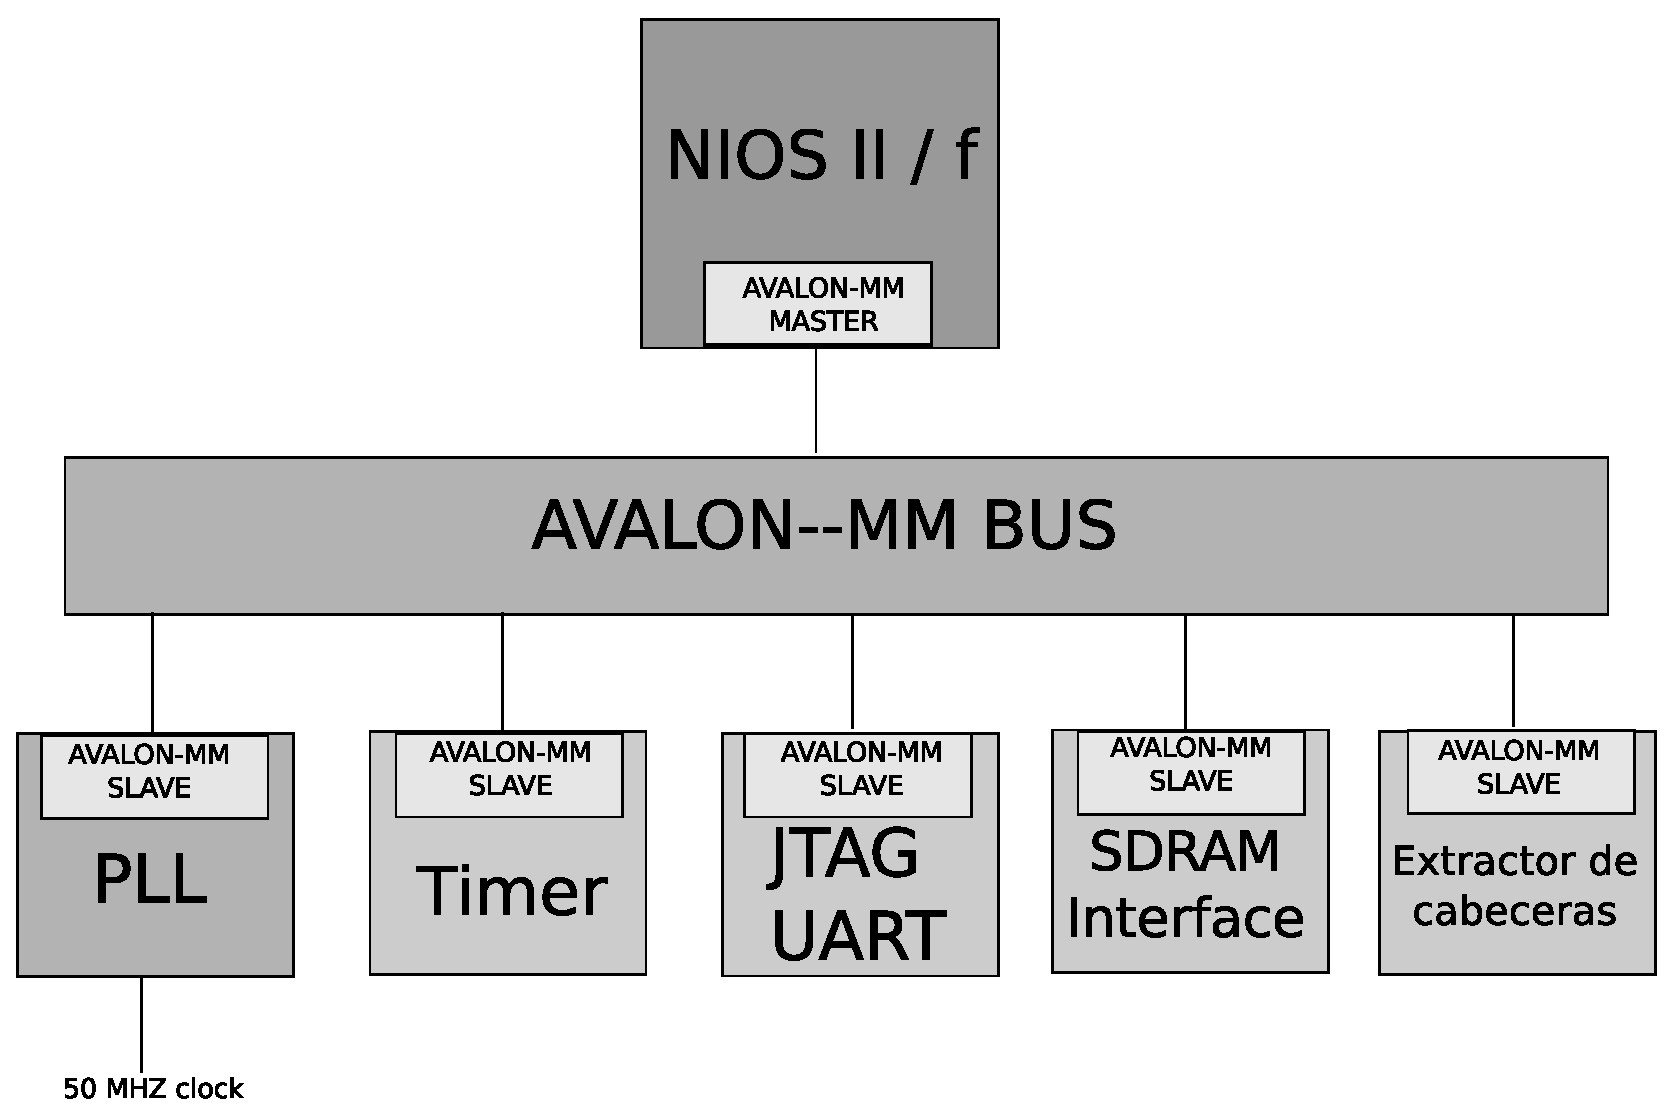
\includegraphics[width=0.80\textwidth]{2-sistema/graf/sistema.eps}
  \caption{Sistema}
  \label{fig}
\end{figure}

A su vez, éste último está conformado por un generador de paquetes Ethernet conectado a una FIFO. Esta está a su vez conectada a un modulo denominado delay buffer, que está conectado al modulo uplink y al write output.. Uplink a su vez está conectado también a write output.

\begin{figure}[h]
  \centering
	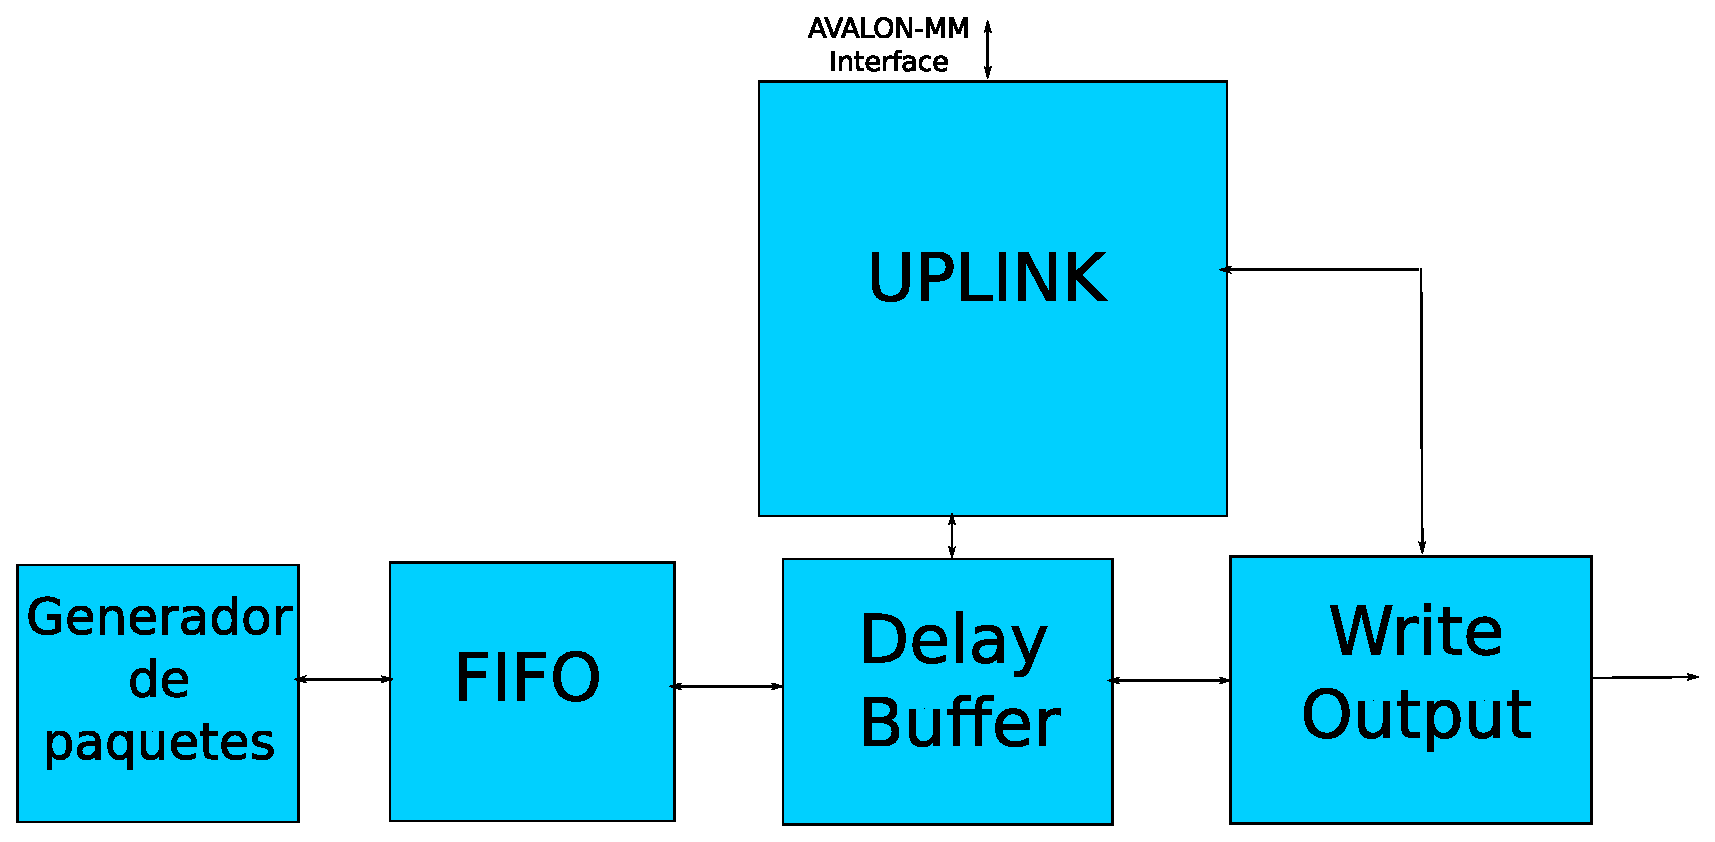
\includegraphics[width=0.80\textwidth]{2-sistema/graf/extractor.eps}
  \caption{Extractor de cabeceras}
  \label{fig}
\end{figure}

Sobre el hardware descrito anteriormente se ejecuta un software de clasificacion de paquetes, que se encuentra almacenado en una memoria RAM.



%\section{Distribucion Lineal}
